
\documentclass[border=3pt,tikz]{standalone}
\usepackage[utf8]{vietnam}
\usetikzlibrary{calc,angles,intersections,shapes.geometric,arrows,decorations.markings,arrows.meta,patterns.meta,patterns}
\usepackage{tikz-3dplot,pgfplots}
\pgfplotsset{compat=1.15}
\usepgfplotslibrary{polar}
\usepackage{amsmath}
\begin{document}
	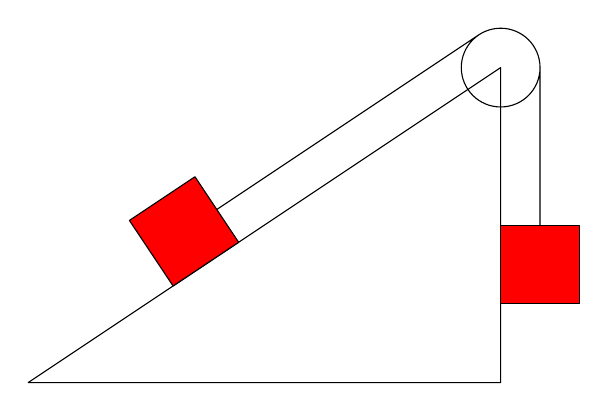
\begin{tikzpicture}[scale=1,line join=round,line cap=round,>=stealth]
	\def\r{4}
	\def\ra{.5}%ban kinh duong tron nho
	\path (0,0)coordinate(A)+(180:1.5*\r)coordinate(B)+(90:\r)coordinate(C);
	\path (B)--(C)--([turn]90:\ra)coordinate(d1)--([turn]90:\r)coordinate(cd1)--([turn]90:\ra)coordinate(cn1)--([turn]-90:2*\ra)coordinate(cn2)--([turn]-90:2*\ra)coordinate(cn3)--([turn]-90:2*\ra)coordinate(cn4);
	\path (A)--(C)--([turn]-90:\ra)coordinate(d2)--([turn]-90:.5*\r)coordinate(cd2)--([turn]-90:\ra)coordinate(an1)--([turn]90:2*\ra)coordinate(an2)--([turn]90:2*\ra)coordinate(an3)--([turn]90:2*\ra)coordinate(an4);
	\draw (A)--(B)--(C)--cycle;
	\draw (d1)--(cd1) (d2)--(cd2) (C)circle(\ra cm);
	\draw[fill=red] (cn1)--(cn2)--(cn3)--(cn4)--cycle;
	\draw[fill=red] (an1)--(an2)--(an3)--(an4)--cycle;
\end{tikzpicture}
\end{document}